% Options for packages loaded elsewhere
\PassOptionsToPackage{unicode}{hyperref}
\PassOptionsToPackage{hyphens}{url}
%
\documentclass[
  ignorenonframetext,
]{beamer}
\usepackage{pgfpages}
\setbeamertemplate{caption}[numbered]
\setbeamertemplate{caption label separator}{: }
\setbeamercolor{caption name}{fg=normal text.fg}
\beamertemplatenavigationsymbolsempty
% Prevent slide breaks in the middle of a paragraph
\widowpenalties 1 10000
\raggedbottom
\setbeamertemplate{part page}{
  \centering
  \begin{beamercolorbox}[sep=16pt,center]{part title}
    \usebeamerfont{part title}\insertpart\par
  \end{beamercolorbox}
}
\setbeamertemplate{section page}{
  \centering
  \begin{beamercolorbox}[sep=12pt,center]{part title}
    \usebeamerfont{section title}\insertsection\par
  \end{beamercolorbox}
}
\setbeamertemplate{subsection page}{
  \centering
  \begin{beamercolorbox}[sep=8pt,center]{part title}
    \usebeamerfont{subsection title}\insertsubsection\par
  \end{beamercolorbox}
}
\AtBeginPart{
  \frame{\partpage}
}
\AtBeginSection{
  \ifbibliography
  \else
    \frame{\sectionpage}
  \fi
}
\AtBeginSubsection{
  \frame{\subsectionpage}
}

\usepackage{amsmath,amssymb}
\usepackage{iftex}
\ifPDFTeX
  \usepackage[T1]{fontenc}
  \usepackage[utf8]{inputenc}
  \usepackage{textcomp} % provide euro and other symbols
\else % if luatex or xetex
  \usepackage{unicode-math}
  \defaultfontfeatures{Scale=MatchLowercase}
  \defaultfontfeatures[\rmfamily]{Ligatures=TeX,Scale=1}
\fi
\usepackage{lmodern}
\ifPDFTeX\else  
    % xetex/luatex font selection
\fi
% Use upquote if available, for straight quotes in verbatim environments
\IfFileExists{upquote.sty}{\usepackage{upquote}}{}
\IfFileExists{microtype.sty}{% use microtype if available
  \usepackage[]{microtype}
  \UseMicrotypeSet[protrusion]{basicmath} % disable protrusion for tt fonts
}{}
\makeatletter
\@ifundefined{KOMAClassName}{% if non-KOMA class
  \IfFileExists{parskip.sty}{%
    \usepackage{parskip}
  }{% else
    \setlength{\parindent}{0pt}
    \setlength{\parskip}{6pt plus 2pt minus 1pt}}
}{% if KOMA class
  \KOMAoptions{parskip=half}}
\makeatother
\usepackage{xcolor}
\newif\ifbibliography
\setlength{\emergencystretch}{3em} % prevent overfull lines
\setcounter{secnumdepth}{-\maxdimen} % remove section numbering

\usepackage{color}
\usepackage{fancyvrb}
\newcommand{\VerbBar}{|}
\newcommand{\VERB}{\Verb[commandchars=\\\{\}]}
\DefineVerbatimEnvironment{Highlighting}{Verbatim}{commandchars=\\\{\}}
% Add ',fontsize=\small' for more characters per line
\usepackage{framed}
\definecolor{shadecolor}{RGB}{241,243,245}
\newenvironment{Shaded}{\begin{snugshade}}{\end{snugshade}}
\newcommand{\AlertTok}[1]{\textcolor[rgb]{0.68,0.00,0.00}{#1}}
\newcommand{\AnnotationTok}[1]{\textcolor[rgb]{0.37,0.37,0.37}{#1}}
\newcommand{\AttributeTok}[1]{\textcolor[rgb]{0.40,0.45,0.13}{#1}}
\newcommand{\BaseNTok}[1]{\textcolor[rgb]{0.68,0.00,0.00}{#1}}
\newcommand{\BuiltInTok}[1]{\textcolor[rgb]{0.00,0.23,0.31}{#1}}
\newcommand{\CharTok}[1]{\textcolor[rgb]{0.13,0.47,0.30}{#1}}
\newcommand{\CommentTok}[1]{\textcolor[rgb]{0.37,0.37,0.37}{#1}}
\newcommand{\CommentVarTok}[1]{\textcolor[rgb]{0.37,0.37,0.37}{\textit{#1}}}
\newcommand{\ConstantTok}[1]{\textcolor[rgb]{0.56,0.35,0.01}{#1}}
\newcommand{\ControlFlowTok}[1]{\textcolor[rgb]{0.00,0.23,0.31}{#1}}
\newcommand{\DataTypeTok}[1]{\textcolor[rgb]{0.68,0.00,0.00}{#1}}
\newcommand{\DecValTok}[1]{\textcolor[rgb]{0.68,0.00,0.00}{#1}}
\newcommand{\DocumentationTok}[1]{\textcolor[rgb]{0.37,0.37,0.37}{\textit{#1}}}
\newcommand{\ErrorTok}[1]{\textcolor[rgb]{0.68,0.00,0.00}{#1}}
\newcommand{\ExtensionTok}[1]{\textcolor[rgb]{0.00,0.23,0.31}{#1}}
\newcommand{\FloatTok}[1]{\textcolor[rgb]{0.68,0.00,0.00}{#1}}
\newcommand{\FunctionTok}[1]{\textcolor[rgb]{0.28,0.35,0.67}{#1}}
\newcommand{\ImportTok}[1]{\textcolor[rgb]{0.00,0.46,0.62}{#1}}
\newcommand{\InformationTok}[1]{\textcolor[rgb]{0.37,0.37,0.37}{#1}}
\newcommand{\KeywordTok}[1]{\textcolor[rgb]{0.00,0.23,0.31}{#1}}
\newcommand{\NormalTok}[1]{\textcolor[rgb]{0.00,0.23,0.31}{#1}}
\newcommand{\OperatorTok}[1]{\textcolor[rgb]{0.37,0.37,0.37}{#1}}
\newcommand{\OtherTok}[1]{\textcolor[rgb]{0.00,0.23,0.31}{#1}}
\newcommand{\PreprocessorTok}[1]{\textcolor[rgb]{0.68,0.00,0.00}{#1}}
\newcommand{\RegionMarkerTok}[1]{\textcolor[rgb]{0.00,0.23,0.31}{#1}}
\newcommand{\SpecialCharTok}[1]{\textcolor[rgb]{0.37,0.37,0.37}{#1}}
\newcommand{\SpecialStringTok}[1]{\textcolor[rgb]{0.13,0.47,0.30}{#1}}
\newcommand{\StringTok}[1]{\textcolor[rgb]{0.13,0.47,0.30}{#1}}
\newcommand{\VariableTok}[1]{\textcolor[rgb]{0.07,0.07,0.07}{#1}}
\newcommand{\VerbatimStringTok}[1]{\textcolor[rgb]{0.13,0.47,0.30}{#1}}
\newcommand{\WarningTok}[1]{\textcolor[rgb]{0.37,0.37,0.37}{\textit{#1}}}

\providecommand{\tightlist}{%
  \setlength{\itemsep}{0pt}\setlength{\parskip}{0pt}}\usepackage{longtable,booktabs,array}
\usepackage{calc} % for calculating minipage widths
\usepackage{caption}
% Make caption package work with longtable
\makeatletter
\def\fnum@table{\tablename~\thetable}
\makeatother
\usepackage{graphicx}
\makeatletter
\def\maxwidth{\ifdim\Gin@nat@width>\linewidth\linewidth\else\Gin@nat@width\fi}
\def\maxheight{\ifdim\Gin@nat@height>\textheight\textheight\else\Gin@nat@height\fi}
\makeatother
% Scale images if necessary, so that they will not overflow the page
% margins by default, and it is still possible to overwrite the defaults
% using explicit options in \includegraphics[width, height, ...]{}
\setkeys{Gin}{width=\maxwidth,height=\maxheight,keepaspectratio}
% Set default figure placement to htbp
\makeatletter
\def\fps@figure{htbp}
\makeatother
\newlength{\cslhangindent}
\setlength{\cslhangindent}{1.5em}
\newlength{\csllabelwidth}
\setlength{\csllabelwidth}{3em}
\newlength{\cslentryspacingunit} % times entry-spacing
\setlength{\cslentryspacingunit}{\parskip}
\newenvironment{CSLReferences}[2] % #1 hanging-ident, #2 entry spacing
 {% don't indent paragraphs
  \setlength{\parindent}{0pt}
  % turn on hanging indent if param 1 is 1
  \ifodd #1
  \let\oldpar\par
  \def\par{\hangindent=\cslhangindent\oldpar}
  \fi
  % set entry spacing
  \setlength{\parskip}{#2\cslentryspacingunit}
 }%
 {}
\usepackage{calc}
\newcommand{\CSLBlock}[1]{#1\hfill\break}
\newcommand{\CSLLeftMargin}[1]{\parbox[t]{\csllabelwidth}{#1}}
\newcommand{\CSLRightInline}[1]{\parbox[t]{\linewidth - \csllabelwidth}{#1}\break}
\newcommand{\CSLIndent}[1]{\hspace{\cslhangindent}#1}

\makeatletter
\makeatother
\makeatletter
\makeatother
\makeatletter
\@ifpackageloaded{caption}{}{\usepackage{caption}}
\AtBeginDocument{%
\ifdefined\contentsname
  \renewcommand*\contentsname{Table of contents}
\else
  \newcommand\contentsname{Table of contents}
\fi
\ifdefined\listfigurename
  \renewcommand*\listfigurename{List of Figures}
\else
  \newcommand\listfigurename{List of Figures}
\fi
\ifdefined\listtablename
  \renewcommand*\listtablename{List of Tables}
\else
  \newcommand\listtablename{List of Tables}
\fi
\ifdefined\figurename
  \renewcommand*\figurename{Figure}
\else
  \newcommand\figurename{Figure}
\fi
\ifdefined\tablename
  \renewcommand*\tablename{Table}
\else
  \newcommand\tablename{Table}
\fi
}
\@ifpackageloaded{float}{}{\usepackage{float}}
\floatstyle{ruled}
\@ifundefined{c@chapter}{\newfloat{codelisting}{h}{lop}}{\newfloat{codelisting}{h}{lop}[chapter]}
\floatname{codelisting}{Listing}
\newcommand*\listoflistings{\listof{codelisting}{List of Listings}}
\makeatother
\makeatletter
\@ifpackageloaded{caption}{}{\usepackage{caption}}
\@ifpackageloaded{subcaption}{}{\usepackage{subcaption}}
\makeatother
\makeatletter
\@ifpackageloaded{tcolorbox}{}{\usepackage[skins,breakable]{tcolorbox}}
\makeatother
\makeatletter
\@ifundefined{shadecolor}{\definecolor{shadecolor}{rgb}{.97, .97, .97}}
\makeatother
\makeatletter
\makeatother
\makeatletter
\makeatother
\ifLuaTeX
  \usepackage{selnolig}  % disable illegal ligatures
\fi
\IfFileExists{bookmark.sty}{\usepackage{bookmark}}{\usepackage{hyperref}}
\IfFileExists{xurl.sty}{\usepackage{xurl}}{} % add URL line breaks if available
\urlstyle{same} % disable monospaced font for URLs
\hypersetup{
  pdftitle={An R client for iRODS},
  pdfauthor={Martin Schobben; Mariana Montes; Christine Staiger; Terrell Russell},
  hidelinks,
  pdfcreator={LaTeX via pandoc}}

\title{An R client for iRODS}
\subtitle{rirods}
\author{Martin Schobben \and Mariana Montes \and Christine
Staiger \and Terrell Russell}
\date{}

\begin{document}
\frame{\titlepage}
\ifdefined\Shaded\renewenvironment{Shaded}{\begin{tcolorbox}[boxrule=0pt, borderline west={3pt}{0pt}{shadecolor}, sharp corners, interior hidden, enhanced, frame hidden, breakable]}{\end{tcolorbox}}\fi

\hypertarget{the-r-ecosystem}{%
\section{The R Ecosystem}\label{the-r-ecosystem}}

\begin{frame}{Introduction to R}
\protect\hypertarget{introduction-to-r}{}
\begin{itemize}
\tightlist
\item
  Emphasis on statistics and visualization of data
\item
  Used by researchers and industry
\item
  Open sourced, active useRs community (26,644 packages)
\end{itemize}

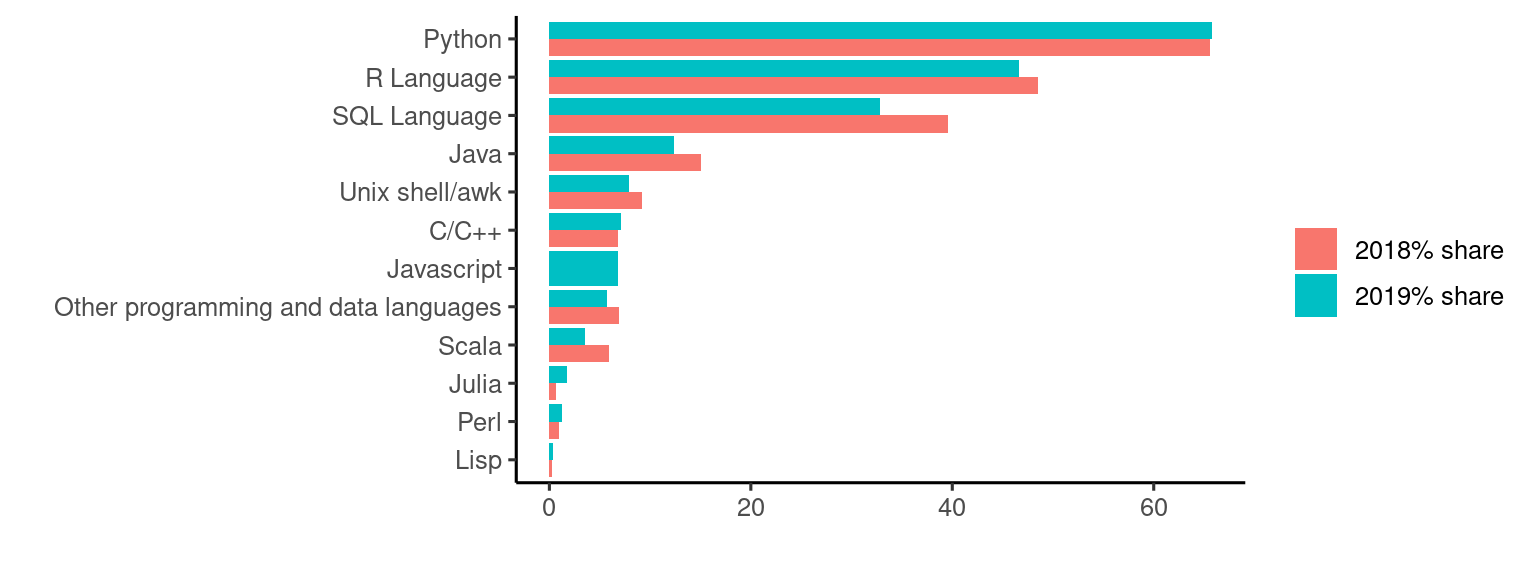
\includegraphics{rirods_ugm_2023_files/figure-beamer/kdnuggest, options-1.pdf}

\note{\begin{itemize}
\tightlist
\item
  Functional programming, or is it? technically not as function don't
  have to pure and can have side effects
\item
  Data is based on a poll with 1800 participants -\textgreater{} which
  program do they use as Data Science platforms
\end{itemize}}
\end{frame}

\begin{frame}[fragile]{Why R?}
\protect\hypertarget{why-r}{}
\begin{itemize}
\tightlist
\item
  Creating reproducible workflows

  \begin{itemize}
  \tightlist
  \item
    Scripted analysis
  \item
    Literate programming (``Rmarkdown'' and ``Quarto'')
  \end{itemize}
\end{itemize}

\emph{Never again wonder what method did I use to center variable
``foo'' in my regression model \ldots{} ?}

\begin{itemize}
\tightlist
\item
  But what about the data itself?

  \begin{itemize}
  \tightlist
  \item
    Centralized, relational, tabular databases
  \end{itemize}
\end{itemize}

\emph{SQLite, MySQL, PostgreSQL, MonetDB with \texttt{DBI} package}

\note{\begin{itemize}
\tightlist
\item
  Relational db
\item
  Reformatting required
\item
  What about non-relational
\item
  Can we store R objects just as they are?
\end{itemize}}
\end{frame}

\begin{frame}[fragile]{Why iRODS?}
\protect\hypertarget{why-irods}{}
\begin{itemize}
\tightlist
\item
  Freedom from strict formatting requirements
\item
  Less data transformations mean higher productivity
\end{itemize}

\begin{codelisting}

\caption{\texttt{irods_ugm2023_bmi_example.R}}

\begin{Shaded}
\begin{Highlighting}[]
\CommentTok{\# height (cm)}
\NormalTok{x }\OtherTok{\textless{}{-}} \FunctionTok{c}\NormalTok{(}\DecValTok{151}\NormalTok{, }\DecValTok{174}\NormalTok{, }\DecValTok{138}\NormalTok{, }\DecValTok{186}\NormalTok{, }\DecValTok{128}\NormalTok{, }\DecValTok{136}\NormalTok{, }\DecValTok{179}\NormalTok{, }\DecValTok{163}\NormalTok{, }\DecValTok{152}\NormalTok{, }\DecValTok{131}\NormalTok{)}
\CommentTok{\# weight (kg)}
\NormalTok{y }\OtherTok{\textless{}{-}} \FunctionTok{c}\NormalTok{(}\DecValTok{63}\NormalTok{, }\DecValTok{81}\NormalTok{, }\DecValTok{56}\NormalTok{, }\DecValTok{91}\NormalTok{, }\DecValTok{47}\NormalTok{, }\DecValTok{57}\NormalTok{, }\DecValTok{76}\NormalTok{, }\DecValTok{72}\NormalTok{, }\DecValTok{62}\NormalTok{, }\DecValTok{48}\NormalTok{)}
\CommentTok{\# linear regression body mass index}
\NormalTok{BMI }\OtherTok{\textless{}{-}} \FunctionTok{lm}\NormalTok{(y }\SpecialCharTok{\textasciitilde{}}\NormalTok{ x) }
\FunctionTok{summary}\NormalTok{(BMI)}
\end{Highlighting}
\end{Shaded}

\end{codelisting}

\begin{verbatim}

Call:
lm(formula = y ~ x)

Residuals:
    Min      1Q  Median      3Q     Max 
-6.3002 -1.6629  0.0412  1.8944  3.9775 

Coefficients:
             Estimate Std. Error t value Pr(>|t|)    
(Intercept) -38.45509    8.04901  -4.778  0.00139 ** 
x             0.67461    0.05191  12.997 1.16e-06 ***
---
Signif. codes:  0 '***' 0.001 '**' 0.01 '*' 0.05 '.' 0.1 ' ' 1

Residual standard error: 3.253 on 8 degrees of freedom
Multiple R-squared:  0.9548,    Adjusted R-squared:  0.9491 
F-statistic: 168.9 on 1 and 8 DF,  p-value: 1.164e-06
\end{verbatim}
\end{frame}

\begin{frame}[fragile]{Why iRODS?}
\protect\hypertarget{why-irods-1}{}
\begin{itemize}
\tightlist
\item
  Describing your data with metadata tags
\item
  Making it findable for your peers
\end{itemize}

\emph{What was object \texttt{BMI} again?}
\end{frame}

\begin{frame}[fragile]{Why iRODS?}
\protect\hypertarget{why-irods-2}{}
\begin{codelisting}

\caption{\texttt{irods_ugm2023_bmi_example.R}}

\begin{Shaded}
\begin{Highlighting}[]
\FunctionTok{ils}\NormalTok{(}\AttributeTok{metadata =} \ConstantTok{TRUE}\NormalTok{)}
\end{Highlighting}
\end{Shaded}

\end{codelisting}

\begin{verbatim}

========
metadata
========
/tempZone/home/martin/BMI.rds :
 attribute    value units
 file_type R object   RDS
   content  content      


==========
iRODS Zone
==========
                  logical_path        type
 /tempZone/home/martin/BMI.rds data_object
\end{verbatim}
\end{frame}

\hypertarget{designing-an-r-package}{%
\section{Designing an R package}\label{designing-an-r-package}}

\begin{frame}[fragile]{CRAN Policies}
\protect\hypertarget{cran-policies}{}
\emph{Comprehensive R Archive Network (CRAN)}

\begin{itemize}
\tightlist
\item
  The philosophy

  \begin{itemize}
  \tightlist
  \item
    Portablility: \emph{Happy useRs across the board}
  \item
    Stability: \emph{Stringent requirements for a stable ecosystem}
  \end{itemize}
\item
  What constitutes a good package?

  \begin{itemize}
  \tightlist
  \item
    Tested and well-documented code
  \item
    \texttt{R\ CMD\ check} 50+ tests
  \end{itemize}
\end{itemize}

\note{Tested means it has to run on Linux, macOS and Windows under
different versions of R.}
\end{frame}

\begin{frame}{A Short History of R + iRODS}
\protect\hypertarget{a-short-history-of-r-irods}{}
\begin{itemize}
\tightlist
\item
  Old R package build on the iRODS C++ API (archived)
\item
  New R package build on the iRODS REST API
\end{itemize}

\begin{longtable}[]{@{}lcc@{}}
\toprule\noalign{}
Feature\textbackslash API & iRODS REST & iRODS C++ \\
\midrule\noalign{}
\endhead
\textbf{Portability} & ✓ & ❌ \\
\textbf{Stability} & ✓ & ❌ \\
\bottomrule\noalign{}
\end{longtable}
\end{frame}

\begin{frame}{Global Design}
\protect\hypertarget{global-design}{}
\begin{columns}[T]
\begin{column}{0.5\textwidth}
\begin{itemize}
\tightlist
\item
  Mimic iCommands
\item
  User facing
\item
  Modular and adaptable (e.g.~new REST API)
\end{itemize}
\end{column}

\begin{column}{0.5\textwidth}
\begin{figure}

{\centering 
\includegraphics{pexels-pixabay-262488.jpg}

}

\caption{Photo from \href{https://www.pexels.com}{pexels.com}}

\end{figure}
\end{column}
\end{columns}
\end{frame}

\begin{frame}[fragile]{Interface}
\protect\hypertarget{interface}{}
\begin{longtable}[]{@{}
  >{\raggedright\arraybackslash}p{(\columnwidth - 4\tabcolsep) * \real{0.2329}}
  >{\centering\arraybackslash}p{(\columnwidth - 4\tabcolsep) * \real{0.4658}}
  >{\centering\arraybackslash}p{(\columnwidth - 4\tabcolsep) * \real{0.3014}}@{}}
\toprule\noalign{}
\begin{minipage}[b]{\linewidth}\raggedright
\end{minipage} & \begin{minipage}[b]{\linewidth}\centering
R
\end{minipage} & \begin{minipage}[b]{\linewidth}\centering
iCommands
\end{minipage} \\
\midrule\noalign{}
\endhead
\textbf{Authentication} & \texttt{iauth} & \texttt{iinit} \\
\textbf{Navigation} & \texttt{icd}, \texttt{ils}, \texttt{ipwd} &
\texttt{icd}, \texttt{ils}, \texttt{ipwd} \\
\textbf{Objects} & \texttt{iput}, \texttt{iget}, \texttt{imkdir},
\texttt{irm}, \texttt{isaveRDS}, \texttt{ireadRDS} & \texttt{iput},
\texttt{iget}, \texttt{imkdir}, \texttt{irm} \\
\textbf{Metadata} & \texttt{imeta}, \texttt{iquery} & \texttt{imeta},
\texttt{iquest} \\
\bottomrule\noalign{}
\end{longtable}
\end{frame}

\begin{frame}[fragile]{Implementation}
\protect\hypertarget{implementation}{}
\begin{itemize}
\tightlist
\item
  Curl in R

  \begin{itemize}
  \tightlist
  \item
    R interface to libcurl \emph{curl} (Ooms 2023a)
  \item
    Wrapper \emph{httr2} (Wickham 2023) for \emph{curl} and
    \emph{jsonlite} (Ooms 2023b)
  \end{itemize}
\item
  Development + Testing

  \begin{itemize}
  \tightlist
  \item
    iRODS demo-server

    \begin{itemize}
    \tightlist
    \item
      Terminal: \texttt{docker-compose\ up\ -d\ nginx-reverse-proxy}
    \item
      R console: \texttt{use\_irods\_demo()}
    \end{itemize}
  \item
    Testing with mocking \emph{httptest2} (Richardson 2022)
  \item
    Automatic updates of snapshots with GitHub actions
  \item
    \texttt{R\ CMD\ check} without internet (simulate CRAN checks)
  \end{itemize}
\end{itemize}
\end{frame}

\begin{frame}{Maintenance}
\protect\hypertarget{maintenance}{}
\begin{itemize}
\tightlist
\item
  Source files on the iRODS GitHub organization page
\item
  Website: \url{https://irods.github.io/irods_client_library_rirods}
\item
  Maintainers

  \begin{itemize}
  \tightlist
  \item
    Martin Schobben, Vienna University of Technology, Austria
  \item
    Mariana Montes, KU Leuven, Belgium
  \end{itemize}
\end{itemize}
\end{frame}

\begin{frame}{}
\protect\hypertarget{section}{}
\end{frame}

\begin{frame}[fragile]{Future}
\protect\hypertarget{future}{}
\begin{itemize}
\tightlist
\item
  Submitted to CRAN\\
  \texttt{install.packages("rirods")}
\item
  Publication of blog post on updates ``iRODS4R''
\item
  Upgrade in server side buffer size REST API to several Mb
\end{itemize}
\end{frame}

\begin{frame}[fragile]{Demonstration}
\protect\hypertarget{demonstration}{}
Requirements:

\begin{itemize}
\tightlist
\item
  Remote iRODS server with iRODS C++ REST 0.9.3
\item
  Demo server which requires \texttt{docker} and \texttt{docker-compose}
\item
  \texttt{\textgreater{}=\ R\ 4.1}
\end{itemize}

Case study:

\begin{itemize}
\tightlist
\item
  Data set on iRODS commit history
\item
  \url{https://github.com/FAIReLABS/iRODS4R/blob/main/posts/welcome/data/irods_repos.csv}
\end{itemize}
\end{frame}

\begin{frame}{References}
\protect\hypertarget{references}{}
\hypertarget{refs}{}
\begin{CSLReferences}{1}{0}
\leavevmode\vadjust pre{\hypertarget{ref-curl}{}}%
Ooms, Jeroen. 2023a. \emph{Curl: A Modern and Flexible Web Client for
r}. \url{https://CRAN.R-project.org/package=curl}.

\leavevmode\vadjust pre{\hypertarget{ref-jsonlite}{}}%
---------. 2023b. \emph{Jsonlite: A Simple and Robust JSON Parser and
Generator for r}. \url{https://CRAN.R-project.org/package=jsonlite}.

\leavevmode\vadjust pre{\hypertarget{ref-httptest2}{}}%
Richardson, Neal. 2022. \emph{Httptest2: Test Helpers for Httr2}.
\url{https://CRAN.R-project.org/package=httptest2}.

\leavevmode\vadjust pre{\hypertarget{ref-httr2}{}}%
Wickham, Hadley. 2023. \emph{Httr2: Perform HTTP Requests and Process
the Responses}. \url{https://CRAN.R-project.org/package=httr2}.

\end{CSLReferences}
\end{frame}



\end{document}
